\section{Introduction Philipp}
\subsection{Main Vision}
This software simplifies the process of managing equipment within educational institutions. Users can easily search for and rent essential items, such as laptops and chargers, and lockers to charge their devices.
Meanwhile, administrators benefit from maintenance reminders, devices tracking, and comprehensive reporting tools. All of these contribute to increased efficiency and convenience for all stakeholders.
\subsection{Core Values}
\begin{enumerate}
    \item Sustainability
    \item Equality
    \item Stress-less
\end{enumerate}

\subsection{Goals for the Project}
The application supports a variety of use cases, which are categorized under three main functionalities: Renting, Managing, and Reporting. Each category is designed to address specific operational needs as follows

\section{Core Functionalitys}
\subsubsection{Renting Devices and Lockers}
\begin{itemize}
\item \textbf{Renting Devices:} Users can rent devices through an intuitive interface, which allows them to select, reserve, and access devices based on availability and specific needs.
\item \textbf{Renting Lockers:} The system provides capabilities for users to rent lockers, facilitating a secure and convenient way to store personal or rented devices within the facility.
\end{itemize}

\subsubsection{Managing Devices, Lockers}
\begin{itemize}
\item \textbf{Manage Devices:} Administrators can oversee all device allocations, track device status, and update device information to ensure optimal operational efficiency.
\item \textbf{Manage Lockers:} This feature allows for the management of locker assignments and status, ensuring that lockers are efficiently utilized and maintained.

\end{itemize}

\subsubsection{Reporting and Manage Problems}
\begin{itemize}
\item \textbf{Report Problems:}Users can report any issues they encounter with the devices or lockers, such as malfunctions or access problems. The system ensures that these problems are promptly addressed and resolved by the administrative staff.
\item \textbf{Manage Problems:} Enables the administration to efficiently handle and resolve reported problems related to devices or lockers, improving service quality and user satisfaction.
\end{itemize}

%\subsection{Distribution of work}
\section{Team Composition and Responsibilities}
In this project, members were divided into specific teams based on their expertise and interests. Each team was assigned specific components of the project, ensuring that their distinct expertise contributed to the comprehensive development and integration of the system, while also collaborating effectively to meet the project's overarching goals. This section outlines the team structure, member assignments, and their respective responsibilities. 

\subsection{Workload Definition}

Each team in our project independently defined their own set of work packages using ClickUp, a versatile tool designed to manage task-based work through a Kanban board visualization. This approach allowed every team member to clearly see their tasks and responsibilities, facilitating better planning and coordination. To maintain momentum and ensure continuous alignment with project goals, the teams reviewed the board every three days. These meetings served as mini-sprints, akin to the Scrum methodology, where progress was assessed, and adjustments were made as necessary. This iterative process helped us stay on track and adapt quickly to any challenges or changes in the project's scope.
\clearpage
\subsection{Hardware and 3D Print}
The Hardware and 3D Printing team was led by Felix Huther, with significant contributions from Kandaker Majharul Islam. Felix was primarily responsible for overseeing the design and execution of the hardware components. Kandaker was introduced to programming the arduino device and implemented several smaller functions. This team also integrated the Fast API for real-time data transmission, sending live data to the frontend via ThinkSpeak.

\begin{figure}[htbp]
    \centering
    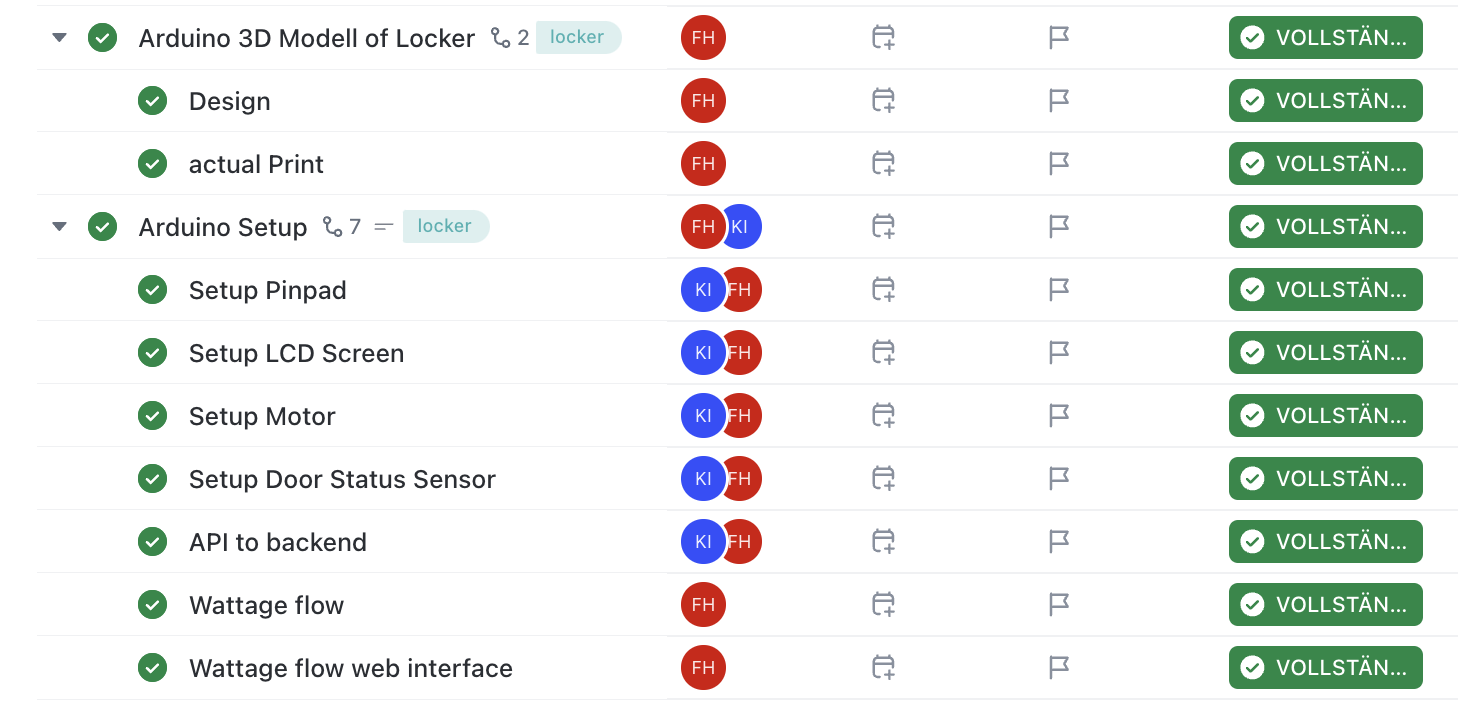
\includegraphics[width=0.9\textwidth]{images/hardware and print.png}
    \caption{Hardware and 3D Model Tasks}
    \label{fig:myimage}
\end{figure}

\subsection{Frontend Development}
Philipp Becker was responsible for the Frontend development, utilizing Vue.js in TypeScript, styled with Tailwind CSS and Vue-Bootstrap. This setup facilitated a robust and responsive user interface. Philipp also integrated the Google API to enhance the functionality and user experience of the application, ensuring seamless interaction with backend services.
\begin{figure}[htbp]
    \centering
    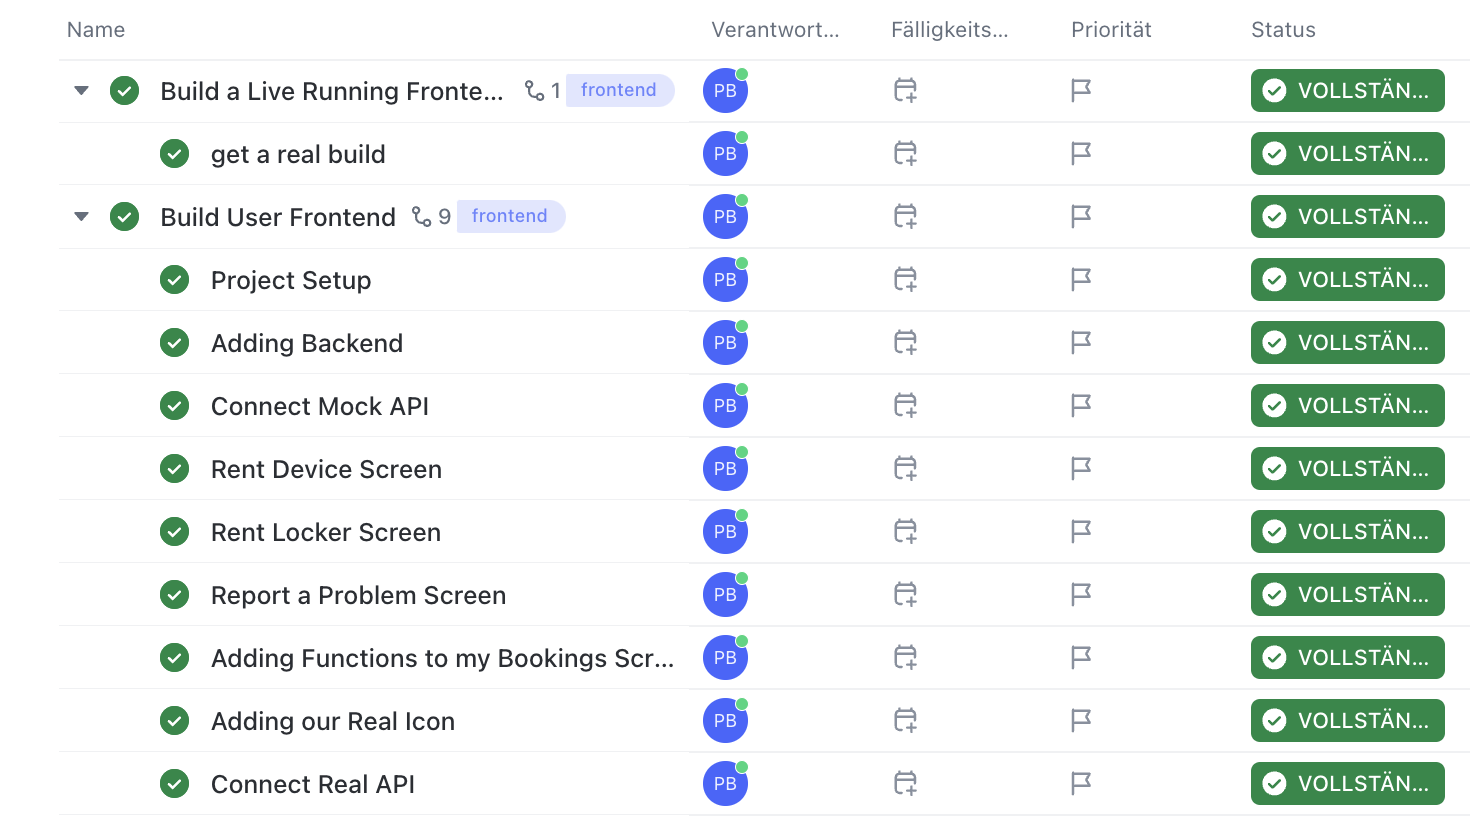
\includegraphics[width=0.9\textwidth]{images/user-frontend.png}
    \caption{User-Frontend Tasks}
    \label{fig:myimage}
    \vspace{1cm}
    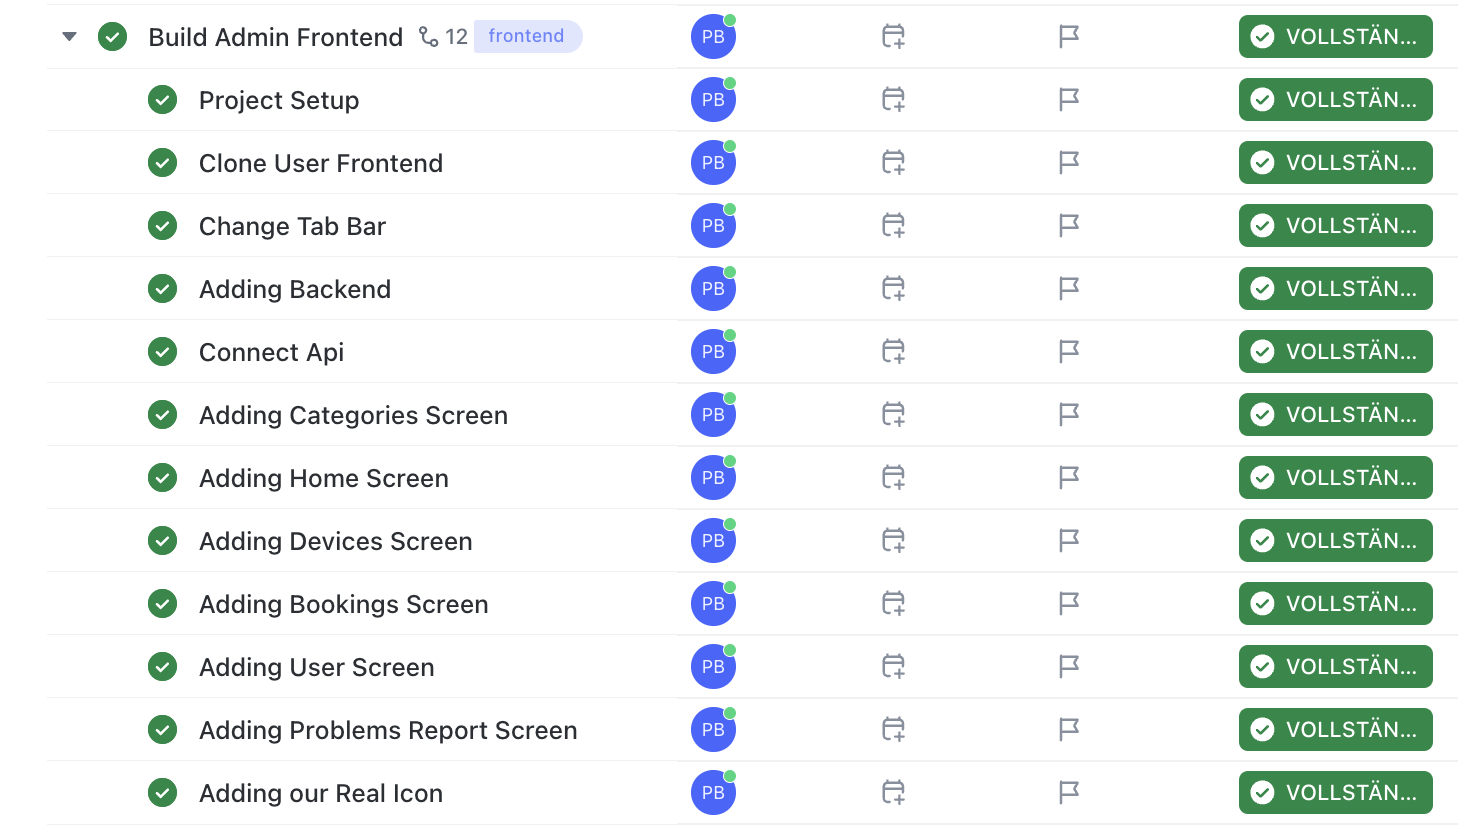
\includegraphics[width=0.8\textwidth]{images/admin-frontend.png}
    \caption{Admin-Frontend Tasks}
    \label{fig:myimage}
\end{figure}
\clearpage
\subsection{Backend Development}
Sven Lepper handled Backend development, employing Alembic with SQL Alchemy as the Object-Relational Mapper (ORM) and PostgreSQL for database management. Fast API was used to create a RESTful interface, enabling efficient communication between the frontend and the database. This setup provided a solid backbone for the application's data handling requirements.

\begin{figure}[h]
    \centering
    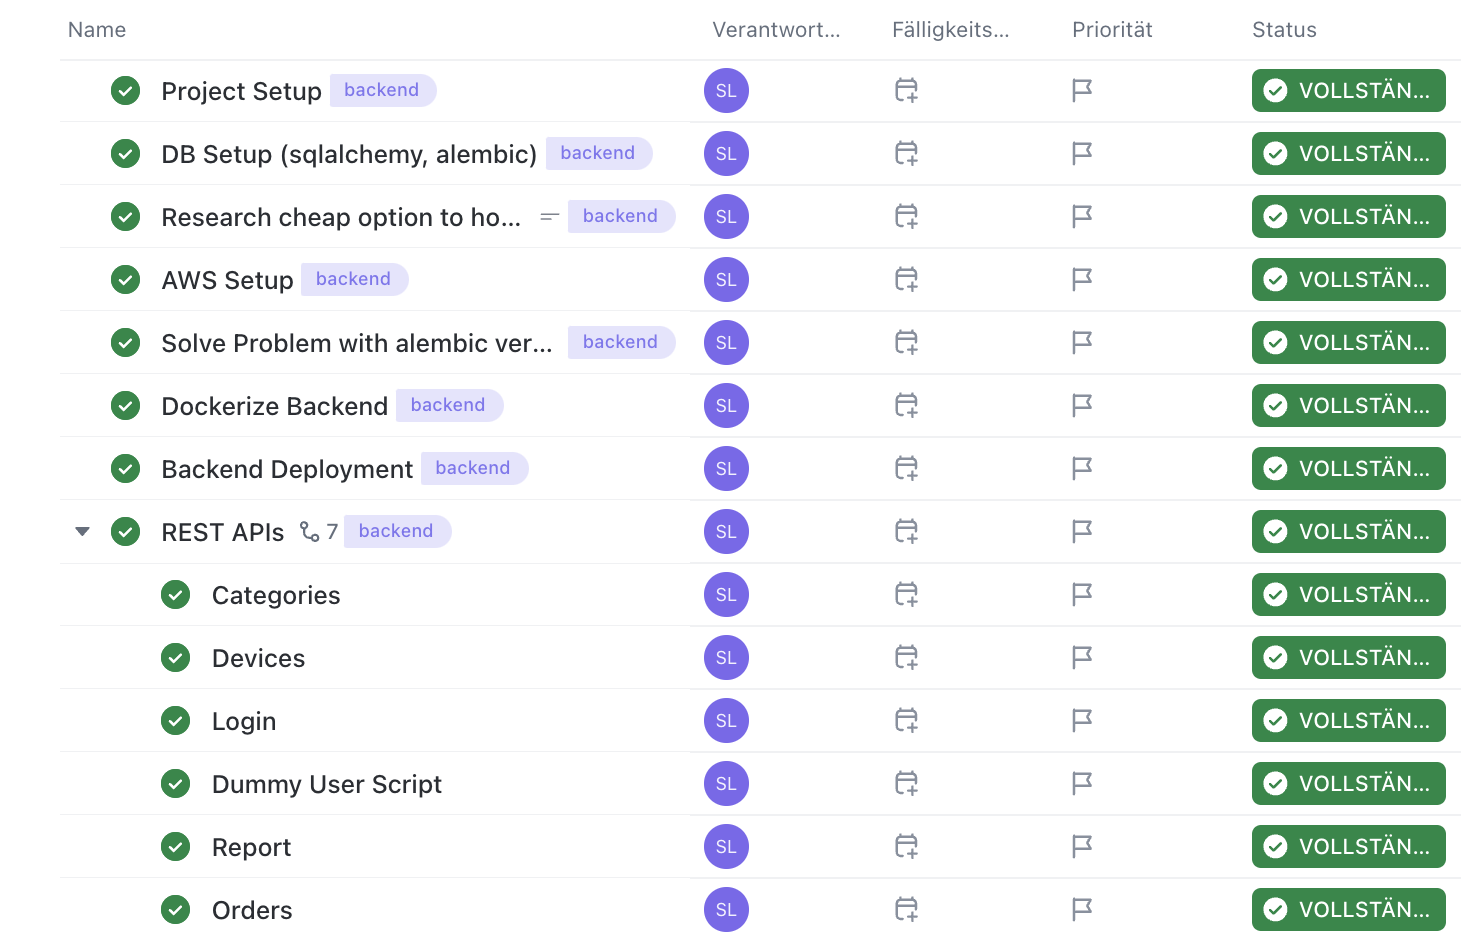
\includegraphics[width=0.9\textwidth]{images/backend.png}
    \caption{User-Frontend Tasks}
    \label{fig:myimage}
\end{figure}
\clearpage
\subsection{API Testing and Hardware Research}
Jingya Zhao took charge of API Testing and Hardware Research. She developed automated tests using Postman, which validated the correctness of data across all backend endpoints. Additionally, Jingya conducted research on live tracking technologies for monitoring the energy usage of devices, which was crucial for the real-time data feature in the project.

\begin{figure}[h]
    \centering
    
\includegraphics[width=0.9\textwidth]{images/R&d.png}
    \caption{Hardware Research Tasks}
    \label{fig:myimage}
    \vspace{1cm}
    
\includegraphics[width=0.9\textwidth]{images/testing.png}
    \caption{API Testing Tasks}
    \label{fig:myimage}
\end{figure}

